\documentclass{beamer}

\usepackage{framed}
\usepackage{graphicx}

\begin{document}

\section{Visualizing the distribution of a dataset}
%===========================================================%
\begin{frame}
	\large
	\noindent \textbf{Visualizing the distribution of a dataset}
	\begin{itemize}
\item When dealing with a set of data, often the first thing you’ll want to do is get a sense for how the variables are distributed.
\item  This chapter of the tutorial will give a brief introduction to some of the tools in seaborn for examining univariate and bivariate distributions. 
\item You may also want to look at the categorical plots chapter for examples of functions that make it easy to compare the distribution of a variable across levels of other variables.
	\end{itemize}

\end{frame}
%=============================================================%
\begin{frame}[fragile]
\begin{framed}
\begin{verbatim}
%matplotlib inline
import numpy as np
import pandas as pd
from scipy import stats, integrate
import matplotlib.pyplot as plt
import seaborn as sns
sns.set(color_codes=True)
np.random.seed(sum(map(ord, "distributions")))
\end{verbatim}
\end{framed}
\end{frame}
%=============================================================%
\section{Plotting univariate distributions}
\begin{frame}[fragile]
The most convenient way to take a quick look at a univariate distribution in seaborn is the distplot() function. By default, this will draw a histogram and fit a kernel density estimate (KDE).

\begin{verbatim}
x = np.random.normal(size=100)
sns.distplot(x);
\end{verbatim}

\begin{figure}
	\centering
	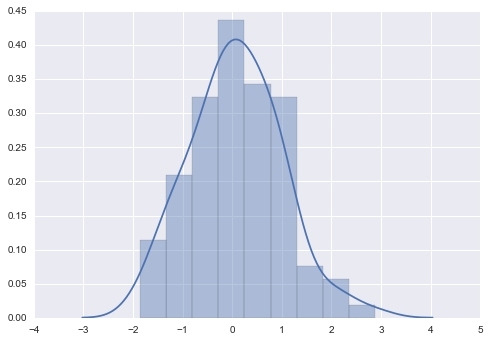
\includegraphics[width=0.7\linewidth]{images/distributions_8_0}
	\caption{}
	\label{fig:distributions_8_0}
\end{figure}

\end{frame}
\section{Histogram}
%===========================================================%
\begin{frame}[fragile]
	\large
\noindent \textbf{Histograms}
\begin{itemize}
\item Histograms are likely familiar, and a hist function already exists in matplotlib. 
\item A histogram represents the distribution of data by forming bins along the range of the data and then drawing bars to show the number of observations that fall in each bin.
\end{itemize}

\end{frame}
%===========================================================%
\begin{frame}[fragile]
	\large
\begin{itemize}
\item To illustrate this, let’s remove the density curve and add a rug plot, which draws a small vertical tick at each observation. 
\item You can make the rug plot itself with the rugplot() function, but it is also available in \texttt{distplot()}:
\end{itemize}


sns.distplot(x, kde=False, rug=True);
\begin{figure}
\centering
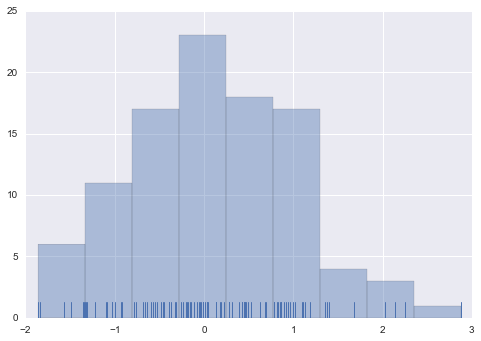
\includegraphics[width=0.7\linewidth]{images/distributions_10_0}
\end{figure}

\end{frame}
%===========================================================%
\begin{frame}[fragile]
When drawing histograms, the main choice you have is the number of bins to use and where to place them. \texttt{distplot()} uses a simple rule to make a good guess for what the right number is by default, but trying more or fewer bins might reveal other features in the data:

\end{frame}
%===========================================================%
\begin{frame}[fragile]
\begin{verbatim}
sns.distplot(x, bins=20, kde=False, rug=True);
\end{verbatim}

\begin{figure}
	\centering
	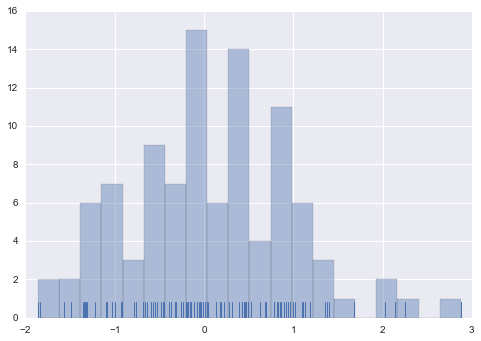
\includegraphics[width=0.7\linewidth]{images/distributions_12_0}
\end{figure}
\end{frame}

\end{document}
